\begin{figure}

  \setlength{\unitlength}{\textwidth}
  \begin{picture}(1,0.3)(0.0,0.6)
    \put(0.025,0.5){\includegraphics[width=0.5\unitlength]{../FnP/gnuplot/mean_power_collapsed_mstar.eps}}
    \put(0.495,0.5){\includegraphics[width=0.5\unitlength]{../FnP/gnuplot/mean_power_collapsed_noshed_mstar.eps}}
    
    \put(-0.01,0.637){\large $\frac{P_{m}}{\rho \mathcal{A}U^3}$}
    
    % \put(0.23,0.48){$\displaystyle\frac{c}{\rho\mathcal{A}U}$} 	
    % \put(0.73,0.48){$\displaystyle\frac{c}{\rho\mathcal{A}U}$}

    \put(0.28,0.48){\massdamp} 	
    \put(0.78,0.48){\massdamp}
    
    \put(0.085,0.709){\small(a)}
    \put(0.555,0.709){\small(b)}
    
  \end{picture}
  
  
  \caption{Mean power as a function of damping factor. Data are presented at $m^*=10$ (\ding{108}), $m^*=20$ (\ding{83}), $m^*=40$ (\ding{115}), $m^*=60$ (+) at Re 165 (a) with and (b) without the shedding term in equation \ref{final_equation_motion}. A reduction of maximum mean power can be observed when $m^*<40$ with shedding while the maximum power is essentially independent of $m^*$ when shedding is disregarded.}
    \label{fig:m_star_collapsed}
\end{figure}



